\documentclass[twocolumn, 10pt,a4j]{jsarticle}
\usepackage{amsmath}
\usepackage[dvipdfmx]{graphicx}
\usepackage{url}
\usepackage[dvipdfmx]{graphicx}
\usepackage{here}
\title{\vspace{-2.5cm}8. 論理回路}
\author{1610581 堀田 大地}
\date{2018/5/17}
\begin{document}
\maketitle{}
\section{目的}
% 目的
トランジスタ,IC等の半導体素子の発展と共に機械システムへのエレクトロニクスの導入が進み,
今やエレクトロニクスと関わりのない機械システムは考えられなくなった.特にコンピュータを始め,
その周辺機器,各種情報機器,NC工作機械, 家電製品等にはディジタル回路が多用されている.そこで,
実際に広く利用されているディジタル用ICを用いて,ディジタル回路,特に論理回路の基礎的事項について実験し,
ディジタルICの使い方,動作,設計法について理解する.
\section{方法}
% 方法
\section{実験項目}
% 実験項目
\subsection{ゲート回路}
% ゲート回路
6種類のゲート回路についての素子名称,動作表,回路の読み方,真理値表,論理式を表4.1に示した.
\subsection{2入力EX-ORゲート}
  % 2入力EX-ORゲート
  \subsubsection{EX-ORの機能}
    % EX-ORの機能
    回路図を図1,動作表,真理値表を表1,2,論理式を(1)に示した.
      % 図1
    \begin{figure}[H]
      \begin{center}
        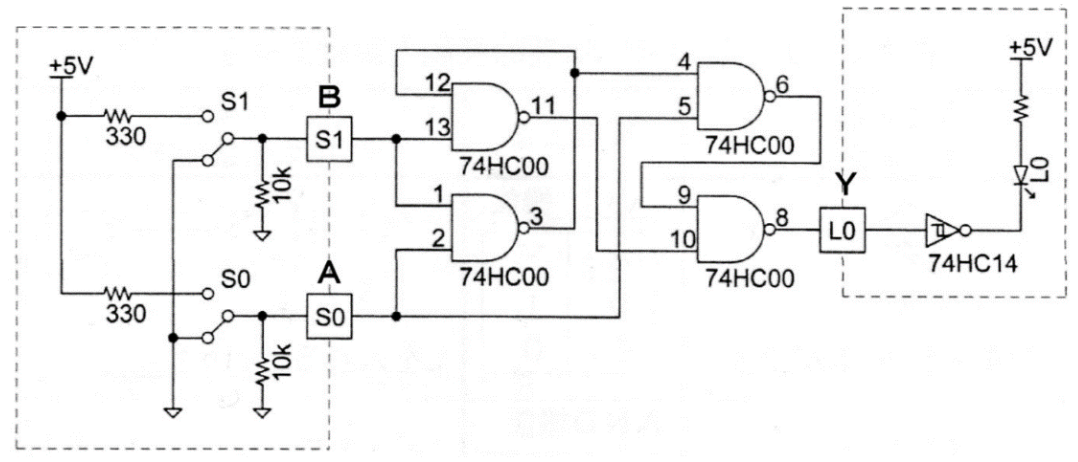
\includegraphics[width=7cm]{../img/ex_or/ex-or_kairo.png}
        \caption{NAND素子4個を用いたEX-OR機能の論理式}
      \end{center}
    \end{figure}
      % 表1 
    \begin{table}[]
      \centering
      \caption{EX-ORの回路の動作表.入力のHはスイッチON,出力のHはLEDの点灯を表す}
      \label{my-label}
      \begin{tabular}{l|ll|l}
            & 入力                      &    & 出力 \\ \hline
        接続端子 & \multicolumn{1}{l|}{$S_{0}$} & $S_{1}$ & $L_{0}$ \\ \hline
        端子名  & \multicolumn{1}{l|}{A}  & B  & Y  \\ \hline
            & \multicolumn{1}{l|}{L}  & L  & L  \\
        電圧   & \multicolumn{1}{l|}{L}  & H  & H  \\
            & \multicolumn{1}{l|}{H}  & L  & H  \\
            & \multicolumn{1}{l|}{H}  & H  & L 
      \end{tabular}
    \end{table}
      % 表2
    \begin{table}[]
      \centering
      \caption{EX-OR機能の真理値表}
      \label{my-label}
      \begin{tabular}{l|ll|l}
            & 入力                     &   & 出力 \\ \hline
        端子名 & \multicolumn{1}{l|}{A} & B & Y  \\ \hline
            & \multicolumn{1}{l|}{0} & 0 & 0  \\
        真理値 & \multicolumn{1}{l|}{0} & 1 & 1  \\
            & \multicolumn{1}{l|}{1} & 0 & 1  \\
            & \multicolumn{1}{l|}{1} & 1 & 0 
      \end{tabular}
    \end{table}
    
    \begin{center}
      $Y = A・\overline{B} + \overline{A} + B = A \oplus B$\quad(1)
    \end{center}
  \subsubsection{考察}
   % 考察
   実験では,$S_{0}$と$S_{1}$のうち1方がオンの状態でのみ,LEDが光っていたことので,動作を確認できた.
   また,LEDの光り方により,回路の機能は理解できた.
  \subsubsection{課題}
    % 課題
    実験で用いた回路を正論理/負論理のNAND素子を使って書き換えた回路を図に示した.
    この課題では,図の回路の出力YがEX-OR機能であることを示した.
    C,$\overline{D}$,$\overline{E}$での論理式を次式(2)-(5)に示した.
    % 図2
    \begin{figure}[H]
      \begin{center}
        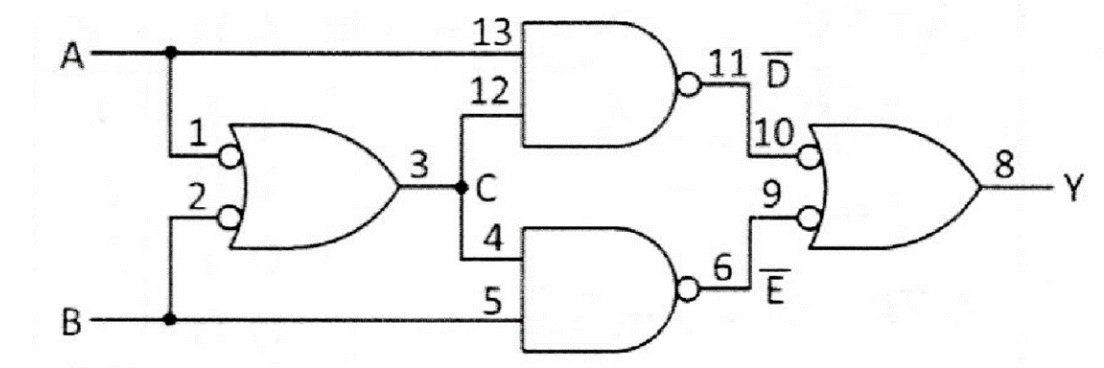
\includegraphics[width=7cm]{../img/ex_or/nand_ex_or_kairo.png}
        \caption{正論理/負論理のNAND素子を使って作ったEX-OR回路}
      \end{center}
    \end{figure}
      % 数式
    \begin{center}
        $C = \overline{A} + \overline{B}$\quad(2) \\
        $\overline{D} = A・C = A・(\overline{A} + \overline{B}) = A・\overline{B}$\quad(3) \\
        $\overline{E} = B・C = B・(\overline{A} + \overline{B}) = \overline{A}・B$\quad(4) \\
        $Y = \overline{D}+\overline{E}=A・\overline{B}+\overline{A}・B=A \oplus B$\quad(5) \\
    \end{center}
    よって, (5)より,図がEX-OR機能であることが示された.
\subsection{デコーダとエンコーダ}
% デコーダとエンコーダ
  \subsubsection{デコーダの機能}
  % デコーダの機能
  デコーダ回路は,2桁の2進数スイッチを使って入力し,10進数の0から3を表すLEDに"1(H)"を出力する.
  すなわち対応するLEDが点灯する回路である.
  回路図を図3,デコーダの動作表,真理値表を表3,4に示した.
   % 図3
  \begin{figure}[H]
    \begin{center}
      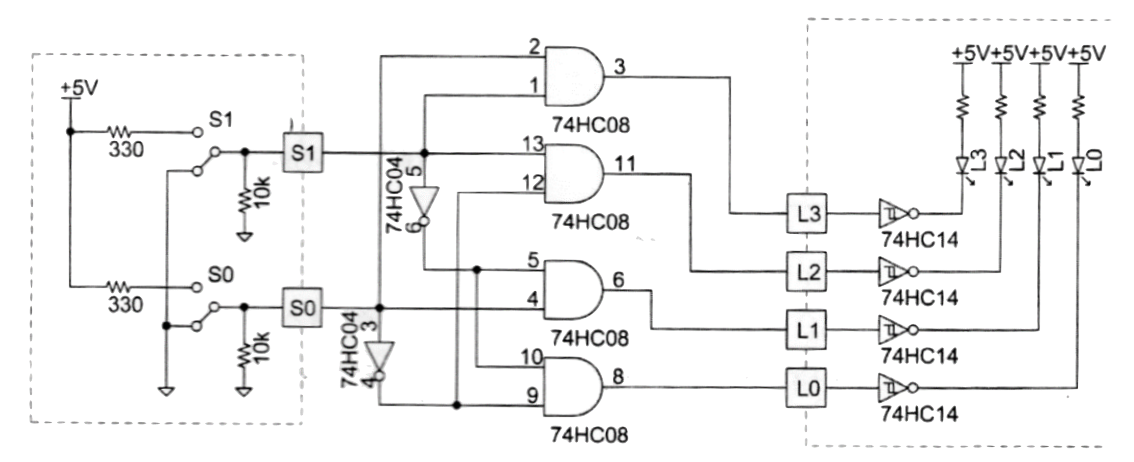
\includegraphics[width=7cm]{../img/decoda/input2_decoda.png}
      \caption{2入力4出力デコーダの回路図}
    \end{center}
  \end{figure}
  % 表3
  \begin{table}[H]
    \centering
    \caption{デコーダの動作表.入力のHはスイッチON,出力のHはLEDの点灯を表す.}
    \label{my-label}
      \begin{tabular}{l|ll|llll}
          & 入力 &    & 出力 &    &    &    \\ \hline
      端子名 & $S_{1}$ & $S_{0}$ & $L_{0}$ & $L_{1}$ & $L_{2}$ & $L_{3}$ \\ \hline
          & L  & L  & H  & L  & L  & L  \\
      電圧  & L  & H  & L  & H  & L  & L  \\
          & H  & L  & L  & L  & H  & L  \\
          & H  & H  & L  & L  & L  & H 
      \end{tabular}
  \end{table}
  % 表4
  \begin{table}[H]
    \centering
    \caption{デコーダの真理値表.
    入力の上位ビット,下位ビットを$S_{1}$,$S_{0}$,出力を$L_{x}$(x=0-3)が表す.}
    \label{my-label}
      \begin{tabular}{l|ll|llll}
          & 入力 &    & 出力 &    &    &    \\ \hline
      端子名 & S1 & S0 & L0 & L1 & L2 & L3 \\ \hline
          & 0  & 0  & 1  & 0  & 0  & 0  \\
      電圧  & 0  & 1  & 0  & 1  & 0  & 0  \\
          & 1  & 0  & 0  & 0  & 1  & 0  \\
          & 1  & 1  & 0  & 0  & 0  & 1 
      \end{tabular}
  \end{table}

  \subsubsection{考察}
  改めてこの回路の入力と出力の関係が「解読」であることを考察する.$S_{0}$,$S_{1}$の2入力4通りの組み合わせから,
  4つの出力が生まれる構造があり,出力結果を見るだけで,入力の信号がわかる.つまり,このことから,入力と出力の関係が「解読」であると言える.
  % 考察
  \subsubsection{課題}
  % 課題
  エンコーダは10進数を2進数に変換する回路である.
  この課題では,10進数から0から3をそれぞれに対応する4つのスイッチ($S_{0}$,$S_{1}$,$S_{2}$,$S_{3}$)
  を使って入力し,2つのLED($L_{0}$,$L_{1}$)を使って2ビットの2進数を出力するエンコーダ回路を
  設計し作成する.
  まず,エンコーダの真理値表を表5に,論理式を(6),(7)に,回路図を図4に示した.
  % 表5
  \begin{table}[H]
    \centering
    \caption{エンコーダの真理値表}
    \label{my-label}
      \begin{tabular}{l|ll|llll}
          & 入力      &         &         &         & 出力      &         \\ \hline
      端子名 & $S_{0}$ & $S_{1}$ & $S_{2}$ & $S_{3}$ & $L_{1}$ & $L_{0}$ \\ \hline
          & 1       & 0       & 0       & 0       & hoge    & hoge    \\
      真理値 & 0       & 1       & 0       & 0       & hoge    & hoge    \\
          & 0       & 0       & 1       & 0       & hoge    & hoge    \\
          & 0       & 0       & 0       & 1       & hoge    & hoge   
      \end{tabular}
  \end{table}
  % 論理式
  \begin{center}
    $L_{0} = S_{1}+S_{3}$\quad(6) \\
    $L_{1} = S_{2}+S_{3}$\quad(7) \\
  \end{center}
  % 図4(TODO: あとでエンコーダ回路を設計する)
\subsection{加算回路}
% 加算回路
  \subsubsection{加算回路の機能}
  \subsubsection{考察}
  \subsubsection{課題}
    \begin{enumerate}
    \item 機能説明
    \item フル・アダーの回路設計
    \item 2桁の2進数の加算回路の設計
    \end{enumerate}
\subsection{ラッチ回路}
% ラッチ回路
  \subsubsection{ラッチ回路の機能}
  \subsubsection{考察}
\subsection{J-Kフリップフロップ回路}
% フリップフロップ回路
  \subsubsection{J-Kフリップフロップ回路の機能}
  \subsubsection{考察}
\subsection{Dフリップフロップ回路}
% Dフリップフロップ回路
  \subsubsection{Dフリップフロップ回路の機能}
  \subsubsection{考察}
\subsection{非同期16進カウンタ回路}
% 非同期16進カウンタ回路
  \subsubsection{非同期16進カウンタ回路の機能}
  \subsubsection{考察}
\section{感想}
% 感想


\begin{thebibliography}{3}
\bibitem{}CT-311S 実習セット(デジタル編)学習の手引き,サンハヤト株式会社
\bibitem{}最新74シリーズIC規格票,CQ出版社
\bibitem{}猪飼國夫,本多中二共著,定本 ディジタルシステムの設計,CQ出版社
\end{thebibliography}
\end{document}